\chapter{Introduction}\label{chap:introduction}
In times where computational tasks are getting more and more computational heavy, many systems require multiple servers/computers to complete tasks. These servers/computers (or also refered to as nodes) are often directly interacting with each other, are decentralized and form a so-called Peer-to-peer network. As depicted in figure \ref{fig:setting} each node consists of a CPU, a memory module and a network interface (to communicate with other nodes). All the nodes are composed to one scalable network. The memory system is modeled as distributed memory scheme, where each node has its own memory module, rather than a shared one, in order to avoid bottlenecks in memory access \cite{ChengzhongFrancis}. Each of the computers is assigned a non-negative workload, which from now on is refered to as load. Loads represent various computational taks such as, CPU usage, memory utilization, or internet traffic. The main objective when applying load balancing algorithms is to balance the state of the network, meaning that each node has the average load of the network. This objective is achieved by combating over- and underloading by redirecting load to alternate nodes in the system. Heavily overloaded nodes may fail to complete the assigned tasks due to overheating. In that sense, load balancing enhances coordination in distributed systems improves scalability and ensures high availability.

\begin{figure}[]
    \centering
    \scalebox{0.3}{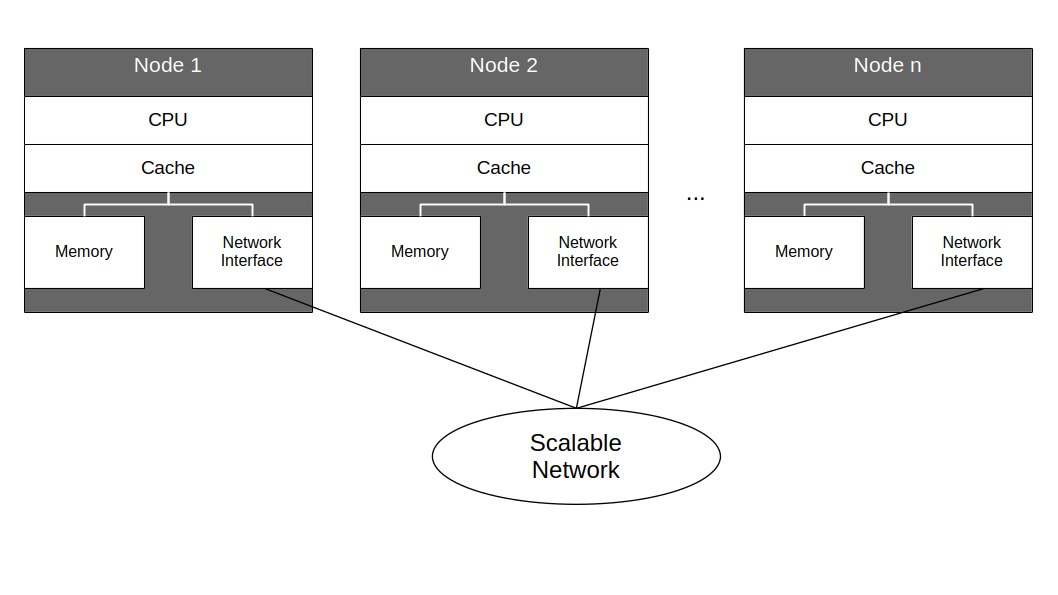
\includegraphics{figures/Diagrams/Setting.png}}
    \caption{Overview of the Setting}
    \label{fig:setting}
\end{figure}

\section{Preliminaries}\label{sec:prelimn}
A graph $G = (V, E \subseteq V \times V)$, where $V := \{v_0, v_1,..., v_{n-1}\}$ are the vertices of $G$ and $E := \{e_1, e_2,...,e_{n-1}\}$ are the edges. The graph may contain only one vertex and zero edges. The number of vertices $|V|$ is often called the order of $G$. A node and a edge are incident, if the node is an endpoint of the edge. The degree of a node is the number of incident edges. If a edge connects two vertices, these vertices are \textit{adjacent} to each other, or also refered to as \textit{neighboring vertices}. A loop is an edge with equal endpoints. Multiple edges are edges with same pair of endpoints. A simple graph has no loops, nor multiple edges. A clique is a set of pairwise adjacent vertices. A path is a simple graph whose vertices can be ordered such that two vertices are adjacent, if and only if they are consecutive in the list. A graph is connected if each pair of vertices in the graph $G$ belongs to a path. A graph is classified as bipartite graph, if the set of graph edges is the union of two disjoint independent sets. If $G$ has a path from node $u$ to node $v$, then the distance from $u$ to v, $d_G(u,v)$ is the shortest length from a $u,v-$path. $\text{diam} (G) := max_{u,v\in V}d_G(u,v)$ is the diameter of a graph. \cite{GraphTheorySchindelhaauer2021} 

\section{Motivation}\label{sec:motivation}
The motivation for this thesis stems from the observed performance discrepancies between the Single-Proposal Deal-Agreement-Based algorithm proposed by Yefim Dinitz, Shlomi Dolev and Manish Kumar \cite{Dinitz2023DAB} and the Push-Pull Sum algorithm described in the paper by Saptadi Nugroho, Alexander Weinmann and Christian Schindelhauer \cite{nugroho2023PushPullSumDataAg} across different network topologies. The obervations were gathered in a the student project with the title "Comparative Analysis of Load Balancing Algorithms in General Graphs" \cite{Bayazitoglu}. Judging from the simulations conducted in the student project, the Push-Pull Sum algorithm seems to perform better in reducing the MSE per round for the complete graph and the star graph compared to the Deal-Agreement-Based algorithm performing better in reducing the MSE per round for the torus grid graph and the ring graph. The simulations were conducted for different network sizes. The network size also played an role in faster convergence.

To address this, the proposed research introduces a novel algorithm, the Adaptive Threshold Push-Pull Sum algorithm that leverages the strengths of both algorithms, creating a Trade-off to mitigate their individual weaknesses. The newly introduced algorithm uses the mechanic of adaptive thresholding, in order to prevent load transfers with low effect in error reduction, since load transfers are pricy operations. By adapting to the structural characteristics of the investigated networks, this new solution aims to achieve robust performance across a wide range of scenarios, bridging the gap between the Deal-Agreement-Based algorithm and the Push-Pull Sum algorithm.

\section{Related Work}\label{sec:relatedwork}
Nugroho et al. \cite{nugroho2023PushPullSumDataAg} proposed the Push-Pull Sum algorithm, which essentially is a composition of two algorithms: the Push-Sum algorithm proposed by David Kempe, Alin Dobra and Johannes Gehrke \cite{kempe2003gossipbasedComp} and the Pull-Sum algorithm. The Push and the Pull mechanics are directly adopted from the Push-Pull Sum algorithm. Nugroho et al. used the mean squared error as a metric to evaluate the performance of their algorithm. In this thesis, I will follow an similar approach. Nugroho et al. conducted their experiments in static general graphs. This research also uses a static graph.  
Dinitz et al. \cite{Dinitz2023DAB} suggested two versions of the Single-Proposal Deal-Agreement-Based algorithm and two versions of a multi-neighbor Load Balancing algorithm, a round robin approach and a self-stabilizing load balancing algorithm. However the only comparable algorithm with ours are the Single-Proposal Deal-Agreement-Based algorithms, from which there exist two variations. One for the contiunous setting and one for the discrete setting. The main difference between these two is that in the contiunous setting any load may be transfered over the edges and in the discrete setting all load transfers must contain integers. For multi-neighbor load balancing the nodes may transfer loads to several neighbors in one round. For the Push-Pull-Sum algorithm this is only the case for the the pull actions where one node responds to every calling node by sending loads back. The self-stabilizing and the round robin approach are asynchronous algorithms, while the Adaptive-Threshold Push-Pull Sum and the Push-Pull Sum algorithms are synchronous algorithm.

\section{Hypothesis}\label{sec:hypothesis}
The Adaptive Threshold Push-Pull Sum load-balancing algorithm, which integrates key features of the Deal-Agreement-Based algorithm and the Push-Pull Sum algorithm, will demonstrate performances that is intermediate between the two in terms of MSE reduction across six distinct network topologies. Specifically, it is expected to perform better than the Deal-Agreement-Based algorithm in high-degree networks and perform better than the Push-Pull Sum algoithm in low-degree networks, achieving a balance that improves overall adaptability and efficiency compared to the both.

This hypothesis will be tested through comparative analysis of the MSE for six distinct topologies (some with different network sizes), demonstrating the algorithm's robustness and scalability across network environments. Model fitting is applied as a analysis technique to see the trend of the data and to be able to make statements regarding the convergence rate. Slopes are computed for three different regions labeled as \textit{Start}, \textit{Middle} and \textit{End}, in order to get details of the performance in specific time frames.

\section{Contribution}\label{sec:contribution}
This study introduces a novel load balancing algorithm that combines the strengths of two established approaches randomized load balancing and deal agreement-based balancing while integrating an adaptive threshold mechanism to enhance performance by adapting to the current state of the network. The load balancing algorithm uses the push and pull mechanics for convergence to a balanced state.